\input{../header.tex}

\setlength{\parindent}{0em}

\begin{document}

\subsection{Implementation}
For the implementation of a Generative Adversarial Network (\textit{GAN}) for the new \textit{MNIST} dataset, a \textit{Discriminator} as well as a \textit{Generator} are used.
\begin{itemize}
  \item Discriminator\\
  The discriminator is trained to distinguish the real \textit{MNIST} images from the generated fake images. 
  For this purpose a small network is used, consisting of dense layers with a number of features from \textit{in\_features} \rightarrow 1024 \rightarrow 512 \rightarrow 128 \rightarrow 1.
  While these layers are split by different dropout layers, the amount of input features is generalized but in this case the image dimension of $28 * 28 =784$ is used.
  Since we have a binary classification problem within the discriminator, the amount of output features is set to 1.
  \item Generator\\
  The generator on the other side is used to generate digits based on random noise. In order to identify and connect most of the features, the use of dropout layers would be counterproductive.
  Therefore, the different dense layers are here split by 1D-batch normalization layers.
  The dense layers have numbers of features from a given latent dimension \textit{latent\_dimension} \rightarrow 256 \rightarrow 512 \rightarrow 1024 \rightarrow 784 (784 being the image dimension of the \textit{MNIST} data).
\end{itemize}.

For the dataset and training I used the following parameters \textit{num\_epochs} = 100, \textit{learning\_rate} = $0.0003$ and \textit{batch\_size} = 32.

\subsection{Results}
The first result is that while the generator loss decreased, the discriminator loss increased (Plots within the ipynb-file).
This suggests that the generator becomes better at fooling the discriminator, causing the discriminator loss to increase.
The problem with the loss for \textit{GAN} is, that they are quite hard to interpret.\\

The loss already stabilized after approximately 30 epochs and then only fluctuated between roughly $0.70$ and $0.85$. On the other side, the quality of the images still improved.
To show this, the generator was tested on a fixed noise in order to compare the digits for each epoch.
In the following three pictures are the generated images of the 0th, 30th and 99th epoch shown.
(The images for all 100 epochs are accessible within the 'images' directory.)
\begin{figure}[H]
  \centering
  \begin{subfigure}[b]{0.32\textwidth}
    \centering
    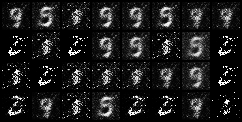
\includegraphics[scale=0.5]{images/fake/fake_epoch_0.png}
    \caption{Generated digits after the 0th epoch.}
  \end{subfigure}
  \hfill
  \begin{subfigure}[b]{0.32\textwidth}
    \centering
    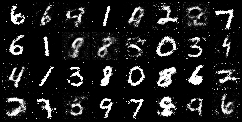
\includegraphics[scale=0.5]{images/fake/fake_epoch_30.png}
    \caption{Generated digits after the 30th epoch.}
  \end{subfigure}
  \hfill
  \begin{subfigure}[b]{0.32\textwidth}
    \centering
    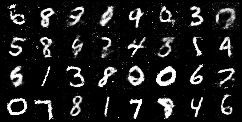
\includegraphics[scale=0.5]{images/fake/fake_epoch_99.png}
    \caption{Generated digits after the 99th epoch.}
  \end{subfigure}
\end{figure}
While the digits in the beginning are extremely noisy and almost every digit was generated as a '9', the digits within the 30th epoch are quite recognizable.
However, there is still an improvement in the image quality during the remaining 69 epochs, mainly through a reduction of noise. 
Even though the loss value is only fluctuating and not decreasing anymore.

This indicates, that the loss alone is not enough to describe the quality of the images.

\subsection{Problems and Improvements}
While the main problems for the training are the missing \textit{early\_stopping} criteria and the changing digits even after the 100th epoch, the main problem for the interpretation were the loss values.
Even though the loss stabilized, the quality of the image still improved, making the number of epochs and the training length quite hard to determine.

The missing \textit{early\_stopping} could be resolved by introducing a new quality measurement. 
One example could be the Wasserstein GANs (\textit{WGAN}), where the discriminator is exchanged by a critic that approximates the Wasserstein distance between the real and fake data distribution. 
By minimizing this distance, it could potentially provide a better \textit{early\_stopping} criteria, than the \textit{GAN} loss values.\\
The fact that some digits are still unrecognizable or still changing might be due to the network for the discriminator and generator.
A deeper network, a hyperparameter optimization or even just more epochs could resolve this problem. 
\end{document}


